\subsection{Soft sheaves}

DEFINITION 5. --- Let \(p\colon E \rightarrow B\) be an étale map. One says that the map \(p\) is soft, or that the étale B-space \((E,p)\) is soft, if every continuous section of \(p\) over a closed subspace of B extends to a continuous section of \(p\) over B.

Let F be a sheaf on B. One says that F is a soft sheaf if the associated étale space (I, p. 50, def. 4) is soft.

Let \(\mathcal{F}\) be a sheaf on B. The sheaf \(\mathcal{F}\) is soft if and only if for every closed set Z of B, every open neighborhood U of Z, and every \(s \in \mathcal{F}(\mathrm{U})\) , there exists \(t \in \mathcal{F}(\mathrm{B})\) and an open neighborhood V of Z contained in U such that \(s \mid \mathrm{V} = t \mid \mathrm{V}\) .

If \(\mathcal{F}\) is a soft sheaf, \(\mathcal{F}(\mathrm{B})\) is nonempty: indeed, the unique section of the étale space \(\mathrm{E}_{\mathcal{F}}\) associated with \(\mathcal{F}\) over \(\varnothing\) extends to a continuous section of \(\mathrm{E}_{\mathcal{F}}\) over B.

Let \(p \colon \mathrm{E} \to \mathrm{B}\) be an étale map and let A be a closed subspace of B. If \(p\) is soft, the map \(p_{\mathrm{A}} \colon \overline{p}^{1}(\mathrm{A}) \to \mathrm{A}\) is soft. Equivalently, if \(\mathcal{F}\) is a soft sheaf on B, the sheaf induced on a closed subspace A is soft.

PROPOSITION 6. --- Let B be a topological space, let \(\mathcal{F}\) be a sheaf on B, and let \((\mathrm{A}_i)_{i\in \mathrm{I}}\) be a locally finite closed covering of B. The sheaf \(\mathcal{F}\) is soft if and only if, for every \(i\in \mathrm{I}\), the induced sheaf \(\mathcal{F}_{\mathrm{A}_i}\) is soft.

The condition is evidently necessary. Let us prove that it is sufficient. Denote by \(p\colon \mathrm{E}\to \mathrm{B}\) the B-étale space \(\mathrm{E}_{\mathcal{F}}\) associated with the sheaf \(\mathcal{F}\) . Let A be a closed subspace of B and \(s\colon \mathrm{A}\to \mathrm{E}\) a continuous section of \(p\) over A; it must be shown that \(s\) has a continuous extension to B. For every subset J of I, set \(\mathrm{A_J} = \bigcup_{i\in \mathrm{J}}\mathrm{A}_i\) ; the set \(\mathrm{A_J}\) is closed in B (TG, I, p. 6, prop. 4).

Let \(\mathcal{S}\) be the set of pairs \((\mathrm{J},t)\) where \(\mathrm{J}\) is a subset of I and \(t\) is a continuous section of E over \(\mathrm{A_J}\) which coincides with \(s\) on \(\mathrm{A} \cap \mathrm{A_J}\) . Equip \(\mathcal{S}\) with the order relation denoted \(\leqslant\) for which \((\mathrm{J},t) \leqslant (\mathrm{J}',t')\) if \(\mathrm{J} \subset \mathrm{J}'\) and \(t' \mid \mathrm{A_J} = t\) . For \(\sigma = (\mathrm{J},t) \in \mathcal{S}\) , write \(\mathrm{J}_{\sigma} = \mathrm{J}\) and \(t_{\sigma} = t\) . Let us show that the ordered set \(\mathcal{S}\) is inductive. Let S be a totally ordered subset of \(\mathcal{S}\) . Set \(\mathrm{J} = \bigcup_{\sigma \in \mathrm{S}} \mathrm{J}_{\sigma}\) ; this is a subset of I. One then defines a section \(t\) of E over \(\mathrm{A_J}\) by setting \(t(x) = t_{\sigma}(x)\) , if \(x \in \mathrm{A}_{J_{\sigma}}\) ; one therefore has \(t \mid \mathrm{A} \cap \mathrm{A_J} = s\) . Let \(j \in \mathrm{J}\) and let \(\sigma \in S\) such that \(j \in J_{\sigma}\) ; since \(t \mid A_j = t_{\sigma} \mid A_j\) the restriction of \(t\) to \(A_j\) is continuous. It then follows from TG, I, p. 19, prop. 4 that \(t\) is continuous. Thus, (J, t) is an element of \(\mathcal{S}\) ; by construction, it is an upper bound of S. This proves that the set \(\mathcal{S}\) is inductive. It therefore possesses a maximal element (J, t) (E, III, p. 20, th. 2).

Let us argue by contradiction, assuming that \(J \neq I\) . Let i be an element of \(I \setminus J\). Set \(A' = (A_i \cap A) \cup (A_i \cap A_J)\) and define a section \(s'\) of E over \(A'\) by:

\[
s ^ {\prime} (a) = \left\{ \begin{array}{l l} s (a) & \text {for} a \in \mathrm{A} _ {i} \cap \mathrm{A}, \\ t (a) & \text {for} a \in \mathrm{A} _ {i} \cap \mathrm{A} _ {\mathrm{J}}, \end{array} \right.
\]

which is possible since \(s\) and \(t\) coincide on \(\mathrm{A} \cap \mathrm{A}_{\mathrm{J}}\) . Moreover, since \(\mathrm{A}_{i} \cap \mathrm{A}\) and \(\mathrm{A}_{i} \cap \mathrm{A}_{\mathrm{J}}\) are closed, the section \(s'\) is continuous (TG, I, p. 19, prop. 4). By hypothesis, there exists a continuous section \(s_{i}: \mathrm{A}_{i} \to \mathrm{E}\) extending \(s'\) . Since the restrictions of \(s_{i}\) and \(t\) to \(\mathrm{A}_{\mathrm{J}} \cap \mathrm{A}_{i}\) are equal, the map \(t': \mathrm{A}_{\mathrm{J} \cup \{i\}} \to \mathrm{E}\) which coincides with \(t\) on \(\mathrm{A}_{\mathrm{J}}\) and with \(s_{i}\) on \(\mathrm{A}_{i}\) is a continuous section of \(p\) over \(\mathrm{A}_{\mathrm{J} \cup \{i\}}\) , extending \(s| \mathrm{A} \cap \mathrm{A}_{\mathrm{J} \cup \{i\}}\) . One then has \((\mathrm{J}, t) < (\mathrm{J} \cup \{i\}, t')\) , which contradicts the hypothesis that \((\mathrm{J}, t)\) is maximal.

Thus, J = I, hence \(A_{J} = B\) and t is a continuous section of E over B extending s.

COROLLARY 1. --- Let B be a paracompact space, \(\mathcal{F}\) a sheaf on B, and \((\mathrm{U}_i)_{i\in \mathrm{I}}\) an open covering of B. If, for every \(i\in \mathrm{I}\) , the induced sheaf \(\mathcal{F}|\mathrm{U}_i\) is soft, then the sheaf \(\mathcal{F}\) is soft.

Indeed, there exists a locally finite closed covering \((\mathrm{F}_{j})_{j\in\mathrm{J}}\) finer than the covering \((\mathrm{U}_{i})_{i\in\mathrm{I}}\) (TG, IX, p. 49, prop. 4 and p. 48, cor. 1). Consequently, for every \(j\in J\), the sheaf \(\mathcal{F}|F_{j}\) is soft and the proposition implies that the sheaf \(\mathcal{F}\) is soft.

COROLLARY 2. --- Let B be a paracompact space, \(\mathcal{F}\) a sheaf on B, and \((\mathrm{A}_i)_{i\in \mathrm{I}}\) a locally finite closed covering of B. For the sheaf \(\mathcal{F}\) to be soft, it is necessary and sufficient that the following condition be satisfied:

For every \(i \in I\) , every closed subset A of \(A_{i}\) , every open set V of B containing A and every element s of \(\mathcal{F}(V)\) , there exists an open neighborhood U of \(A_{i}\) in B, an element t of \(\mathcal{F}(U)\) and an open neighborhood W of A in B contained in \(U \cap V\) such that \(t | W = s | W\) .

Suppose that the sheaf \(\mathcal{F}\) is soft and let us show that the condition is satisfied. Let \(i\in\mathrm{I}\) , let A be a closed subset of \(\mathrm{A}_{i}\) , let V be an open set of B containing A and let \(s\) be an element of \(\mathcal{F}(\mathrm{V})\) . Set \(s_{0}=\sigma_{\mathcal{F}}(s)\) . It is a continuous section over V of the étale space \(\mathrm{E}_{\mathcal{F}}\) . Since \(\mathrm{A}_{i}\) is closed, A is closed in B and \(s_{0}\mid\mathrm{A}\) extends to a section \(t_{0}\colon\mathrm{B}\to\mathrm{E}_{\mathcal{F}}\) , by definition of a soft sheaf. The sections \(s_{0}\) and \(t_{0}\mid\mathrm{V}\) of the V-étale space \(\mathrm{E}_{\mathcal{F}}\times_{\mathrm{B}}\mathrm{V}\) coincide on A, hence on a neighborhood W of A (I, p. 34, prop. 11, b)).

Conversely, suppose that the condition of the corollary is satisfied. By Proposition 6, it suffices to show that, for every \(i \in I\), the sheaf \(\mathcal{F}_{A_i}\) is soft. Let A be a closed subset of \(A_i\) and let \(s_0\) be a section of the étale space of \(\mathcal{F} | A_i\) over A, that is, a continuous section over A of the étale space \(E_{\mathcal{F}}\) . Since A is closed in B and B is paracompact, \(s_0\) extends to a section \(s\) over a neighborhood V of A in B (I, p. 37, th. 2). By hypothesis, there exists an open neighborhood U of \(A_i\) in B and a section \(t\) of \(E_{\mathcal{F}}\) over U which coincides with \(s\) on a neighborhood of A. The restriction of \(t\) to \(A_i\) is a section of \(\mathcal{F}_{A_i}\) which extends \(s_0\) . The sheaf \(\mathcal{F}_{A_i}\) is therefore soft. By Proposition 6, the sheaf \(\mathcal{F}\) is soft.

\subsection{Structure Sheaves}

Suppose that a species of structure \(\Sigma\) and a notion of \(\sigma\)-morphism relative to this species of structure are given.

Let B be a topological space.

A presheaf \(\mathcal{F}\) on B is said to take values in the species of structure \(\Sigma\) if, for every open set U of B, the set \(\mathcal{F}(\mathrm{U})\) is equipped with a structure of species \(\Sigma\) and the restriction maps are \(\sigma\)-morphisms.

We will say that such a presheaf is a sheaf with values in the species of structure \(\Sigma\) if, moreover, it is a sheaf of sets.

If \(\mathcal{F}\) and \(\mathcal{G}\) are presheaves with values in the species of structure \(\Sigma\), one says that a morphism \(\varphi\) is a morphism of presheaves with values in \(\Sigma\) if, for every open set U, the map \(\varphi(\mathrm{U})\) is a \(\sigma\)-morphism.

One will thus speak, for example, of sheaves of groups, of abelian groups, of \(k\)-modules (for a fixed ring \(k\)), of rings, and of \(k\)-algebras (for a fixed commutative ring \(k\)).

The sheaf on B of maps with values in a group (resp. an abelian group, resp. a \(k\)-module, resp. a ring, resp. a \(k\)-algebra) is naturally endowed with a structure of a sheaf of groups (resp. of abelian groups, resp. of \(k\)-modules, resp. of rings, resp. of \(k\)-algebras). If X is a differentiable manifold of class \(C^{r}\) over R, the sheaf \(\underline{\mathcal{C}}^{r}(\mathrm{X};\mathbf{R})\) of numerical functions of class \(C^{r}\) is a sheaf of R-algebras, and the sheaf on X of sections of class \(C^{r}\) of a vector bundle E over X is a sheaf of R-vector spaces; a differential operator defines a morphism of sheaves of R-vector spaces.

For these species of structure \(\Sigma\), it follows from the construction we have given that the sheaf \(\widetilde{\mathcal{F}}\) associated with a presheaf \(\mathcal{F}\) with values in the species of structure \(\Sigma\) (of groups, of abelian groups, of \(k\)-modules, of rings, of \(k\)-algebras) is a sheaf with values in this kind of structure, and that the canonical morphism \(j_{\mathcal{F}}: \mathcal{F} \to \widetilde{\mathcal{F}}\) is a morphism of presheaves with values in the species of structure \(\Sigma\).

For example, the sheaf on B of maps taking values in a group is naturally endowed with a sheaf-of-groups structure.

Let A and B be topological spaces and let \(u\colon\mathrm{A}\to\mathrm{B}\) be a continuous map. If \(\mathcal{F}\) is a (pre)sheaf on A with values in the species of structure \(\Sigma\), then the same is true of the (pre)sheaf \(u_{*}(\mathcal{F})\), the direct image of the (pre)sheaf \(\mathcal{F}\) under \(u\).

Suppose further that the species of structure \(\Sigma\) is that of groups, abelian groups, \(k\)-modules, rings, or \(k\)-algebras. If \(\mathcal{G}\) is a (pre)sheaf on B with values in the species of structure \(\Sigma\), then the sheaf \(u^{*}\mathcal{G}\) on A, inverse image of the presheaf \(\mathcal{G}\) by the map \(u\), is equipped with a sheaf structure with values in \(\Sigma\). In this case, the adjunction morphisms \(\alpha\) and \(\beta\) are morphisms of presheaves with values in the species of structure \(\Sigma\). In particular, if \(\varphi: \mathcal{G} \to u_{*}\mathcal{F}\) is a morphism of presheaves with values in \(\Sigma\), the same holds for the morphism \(\varphi^{\sharp}\); if \(\psi: u^{*}(\mathcal{G}) \to \mathcal{F}\) is a morphism of presheaves with values in \(\Sigma\), the same holds for the morphism \(\psi^{\flat}\).

\section{COVERINGS}

\subsection{Locally trivial fiber spaces}

Let B be a topological space. If F is a topological space, we call the trivial B-fibered space with fiber type F the B-space \((B \times F, pr_{1})\) .

Let E be a B-space. If there exists a topological space F and a B-isomorphism \(u: E \rightarrow B \times F\), we say that the B-space E is a trivializable B-fibered space and that u is a trivialization of it with fiber type F.

DEFINITION 1. --- Let B be a topological space. Let E be a B-space and let p be its projection. One says that E is a locally trivial B-fibered space if every point of B has a neighborhood V such that \((\overline{p}^{1}(V), p_{V})\) is a trivializable V-fibered space.

Instead of “locally trivial fibered B-space,” one also says “locally trivial fibered space with base B.” If E is a locally trivial fibered B-space, one sometimes says that \((E,B,p)\) is a locally trivial fibration, or, by abuse of language, that p is a locally trivial fibration. One also says that a B-space \((E,p)\) is trivializable over a subset A of B if the A-space \(E_{A}\) induced by \((E,p)\) over A is a trivializable fiber space.

Let E be a locally trivial B-fibered space; denote its projection by p. The set of points a in B for which the fiber \(\overline{p}^{1}(a)\) is empty (resp. nonempty) is open. The image of p is therefore an open and closed subset of B.

Let F be a topological space. If all the fibers of E are homeomorphic to F, then E is said to be a locally trivial B-fibered space with fiber type F.

Remarks. --- 1) Let (E, p) be a locally trivial fiber bundle over B, and let A be a subset of B. The A-space \(\mathrm{E}_{\mathrm{A}} = (\stackrel{-1}{p}(\mathrm{A}), p_{\mathrm{A}})\) deduced from E by passing to subspaces is a locally trivial fiber space. If E is trivializable, then so is \(E_{A}\) .

Indeed, for every point \(a\) of A, there exists an open neighborhood U of \(a\) in B, a topological space F and a U-isomorphism \(g\colon \overline{p}^{1}(\mathrm{U})\to \mathrm{U}\times \mathrm{F}\) . The map \(g\) induces an \((\mathrm{A}\cap \mathrm{U})\) -isomorphism of \(\overline{p}_{\mathrm{A}}^{-1}(\mathrm{A}\cap \mathrm{U})\)

onto \((\mathrm{A}\cap\mathrm{U})\times\mathrm{F}\) , which proves that \(E_{A}\) is a locally trivial fibered A-space.

\begin{enumerate}
\def\labelenumi{\arabic{enumi})}
\setcounter{enumi}{1}
\tightlist
\item
  Let \((\mathrm{E}, p)\) be a B-space and let \((\mathrm{E}_{i})_{i \in \mathrm{I}}\) be a partition of E consisting of open sets.
\end{enumerate}

If each of the B-spaces \((\mathrm{E}_{i}, p \mid \mathrm{E}_{i})\) is a trivializable fiber space, E is a trivializable B-fibered space. Indeed, for each \(i \in I\), let \(F_{i}\) be a topological space such that the B-spaces \((\mathrm{E}_{i}, p \mid \mathrm{E}_{i})\) and \((\mathrm{B} \times \mathrm{F}_{i}, \mathrm{pr}_{1})\) are isomorphic. Then the B-space \((\mathrm{E}, p)\) is isomorphic to \((\mathrm{B} \times \mathrm{F}, \mathrm{pr}_{1})\), where F is the topological sum space of the family \((\mathrm{F}_{i})_{i \in I}\) .

Suppose the set I is finite. If each of the B-spaces \((\mathrm{E}_{i}, p \mid \mathrm{E}_{i})\) is a locally trivial B-fibered space, the same holds for the B-space E. Indeed, since the set I is finite, each point of B has a neighborhood U over which the B-fibered spaces \(E_{i}\) are all trivializable. By the preceding, the U-space \((\bar{p}^{1}(\mathrm{U}), p_{\mathrm{U}})\) is then a trivializable fiber bundle.

\subsection{Coverings}

DEFINITION 2. --- A covering is called a locally trivial fiber space all of whose fibers are discrete.

Instead of saying that a B-space E is a covering, one also says that E is a covering of B.

Let E be a B-space, denote by p its projection; let A be a subset of B. If E is a covering of B, the fibers of p are discrete, hence those of \(p_{\mathrm{A}} \colon \overline{p}^{1}(\mathrm{A}) \to \mathrm{A}\) also, and the locally trivial fibered A-space ( \(\overline{p}^{1}(\mathrm{A}), p_{\mathrm{A}}\) ) is a covering.

PROPOSITION 1. --- Let B and E be topological spaces, and let \(p\colon \mathrm{E}\to \mathrm{B}\) be a map. The following conditions are equivalent:

\begin{enumerate}
\def\labelenumi{(\roman{enumi})}
\item
  The map p is continuous and the B-space (E,p) is a trivializable covering.
\item
  There exists a partition \((\mathrm{V}_{i})_{i\in\mathrm{I}}\) of E consisting of open sets such that, for every \(i\in I\), the map \(p\mid V_{i}\colon V_{i}\to B\) is a homeomorphism.
\end{enumerate}

Suppose that condition (i) is satisfied, and let \(g \colon \mathrm{E} \to \mathrm{B} \times \mathrm{F}\) be a trivialization of the B-space \((\mathrm{E}, p)\), of fiber type F. Consequently, F is a discrete topological space and the sets \(\mathrm{V}_i = g^{-1}(\mathrm{B} \times \{i\})\), for \(i \in F\), form a partition of E consisting of open sets. For every \(i\), the map \(p \mid V_i \colon V_i \to B\) is a homeomorphism, with inverse homeomorphism the map \(x \mapsto g^{-1}(x, i)\), whence condition (ii).

Conversely, suppose that condition (ii) is satisfied. The map p is then continuous. Consider the map from E into \(B \times I\) that sends \(x \in E\) to the pair \((p(x), i)\), where i is the unique element of I such that \(x \in V_i\). If I is equipped with the discrete topology, condition (ii) means that this map is a B-isomorphism and the B-space \((E, p)\) is a trivializable covering.

COROLLARY 1. --- Let B and E be topological spaces and let \(p\colon \mathrm{E}\to \mathrm{B}\) be a map. For E, equipped with the map \(p\), to be a covering of B, it is necessary and sufficient that, for every point \(a\) of B, there exists an open neighborhood U of \(a\) and a partition \((\mathrm{V}_i)_{i\in \mathrm{I}}\) of \(\overline{p}^{1}(\mathrm{U})\) formed by open sets of E such that, for every \(i\in \mathrm{I}\), the map \(p\) induces a homeomorphism of \(\mathrm{V}_i\) onto U.

Remark. --- Let B be a topological space. Let E be a B-space and let p be its projection. If E is a covering of B, it follows from Corollary 1 above that the map p is étale (I, p. 28, def. 2) and separated (I, p. 25, prop. 1, (iii)). These conditions are not, however, sufficient to ensure that E is a covering. Consider, for example, an open set U of B. The canonical injection i: U → B is étale and separated. For the B-space (U, i) to be a covering, it is necessary and sufficient that the open set U be also closed.

COROLLARY 2. --- Let B be a topological space, let E be a B-space and let p be its projection. Suppose that p is étale and separated and that the space B is connected. For E to be a trivializable covering of B, it is necessary and sufficient that, for every point x of E, there exists a continuous section s: B → E of p such that \(s(p(x)) = x\).

This is obviously necessary. Conversely, for any continuous section \(s\) of \(p\), the set \(s(\mathrm{B})\) is open and the map \(p\) induces a homeomorphism of \(s(\mathrm{B})\) onto B (I, p. 30, cor. 3 of prop. 6). Moreover, as \(s\) ranges over the set \(\mathcal{S}(\mathrm{B};\mathrm{E})\) of sections of \(p\), the sets \(s(\mathrm{B})\) are pairwise disjoint, since B is connected (I, p. 34, cor. 1 of prop. 11). It then follows from Proposition 1 that if the sets \(s(\mathrm{B})\) cover E, the space E is a trivializable covering of B.

\subsection{Products and fiber products}

PROPOSITION 2. --- Let B and B' be topological spaces, let (E, p) be a B-space and let (E', p') be a B'-space. Suppose that E and E' are locally trivial fibered spaces (resp. coverings). Then the space E × E', equipped with the map p × p': E × E' → B × B', is a locally trivial fibered space (resp. a covering) with base B × B'. If E and E' are trivializable, then so is E × E'.

Suppose first that the B-space E and the B'-space E' admit trivializations \(g: E \to B \times F\) and \(g': E' \to B' \times F'\). The composite of the homeomorphism \(g \times g'\) of \(E \times E'\) onto \((B \times F) \times (B' \times F')\) with the canonical homeomorphism of \((B \times F) \times (B' \times F')\) onto \((B \times B') \times (F \times F')\) is a trivialization of the \(B \times B'\)-space \(E \times E'\), with fiber type \(F \times F'\). If F and \(F'\) are discrete spaces, the space \(F \times F'\) is also discrete.

In the general case, for any point \((a, a')\) of \(B \times B'\), there exists a neighborhood U of a in B and a neighborhood \(U'\) of \(a'\) in B' such that the U-space \(E_{U}\) and the \(U'\)-space \(E_{U'}\) are trivializable. It follows from the preceding that the \(B \times B'\)-space \(E \times E'\) is trivializable over \(U \times U'\). It is therefore a locally trivial fibered space with base \(B \times B'\). Its fibers are discrete if E and \(E'\) are coverings, whence the proposition.

Note that, if \((p_{i} \colon \mathrm{E}_{i} \to \mathrm{B}_{i})_{i \in \mathrm{I}}\) is a family of locally trivial fiber spaces, or even of coverings, the product space \(\prod_{i \in I} E_{i}\) endowed with the map \((p_{i})_{i \in I}\) is not necessarily a locally trivial fiber space with base \(\prod_{i \in I} B_{i}\) (I, p. 145, exerc. 3).

COROLLARY 1. --- Let A be a topological space, and let B, B' be A-spaces. Let E and E' be locally trivial fibered spaces (resp. coverings) with bases B and B'; denote their projections by p and p'. Then the \(B \times_{A} B'\)-space \(E \times_{A} E'\) obtained from p × p' by passing to subspaces is a locally trivial fibered space (resp. a covering). It is trivializable if E and E' are.

Since the set \(E \times_{A} E'\) is the inverse image of \(B \times_{A} B'\) by the mapping \(p \times p'\) : \(E \times E' \to B \times B'\) , the corollary follows from Proposition 2 and Remark 1 (I, p. 68).

COROLLARY 2. --- Let

\pandocbounded{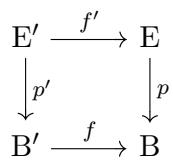
\includegraphics[keepaspectratio]{images/part001_3dd3ce93.jpg}}

a Cartesian square. If (E,p) is a locally trivial B-fibered space (resp. a covering), then (E',p') is a locally trivial fibered space (resp. a covering) with base B', trivializable if (E,p) is.

This follows from Corollary 1, applied with B = A and E' = B'.

COROLLARY 3. --- Let B be a topological space. Let E and E' be locally trivial B-fibered spaces (resp. coverings). Then \(E \times_{B} E'\) is a locally trivial B-fibered space (resp. a covering of B). It is trivializable if E and E' are.

This follows from Corollary 1, applied to the case where A, B, and B' are equal.

PROPOSITION 3. --- Let

\begin{enumerate}
\def\labelenumi{(\arabic{enumi})}
\tightlist
\item
\end{enumerate}

\pandocbounded{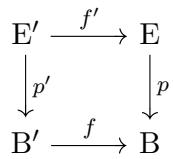
\includegraphics[keepaspectratio]{images/part001_0991252f.jpg}}

a Cartesian square. Suppose that in a neighborhood of every point of B, the map f has a continuous section. Then, if (E', p') is a locally trivial B'-fibered space (resp. a covering), the B-space (E, p) is a locally trivial fibered space (resp. a covering).

We need to prove that every point \(a\) of B has a neighborhood U such that the U-space induced by \((\mathrm{E}, p)\) over U is a locally trivial fibered space (resp. a covering). Take U to be a neighborhood of \(a\) over which there exists a continuous section \(s\) of \(f\). Denote by \(i: \mathrm{U} \to \mathrm{B}\) and \(j: \overline{p}^{-1}(\mathrm{U}) \to \mathrm{E}\) the canonical injections. Since square (1) is Cartesian, there exists a unique continuous map \(s^{\prime}\colon \overline{p}^{1}(\mathrm{U})\to \mathrm{E}^{\prime}\) such that \(f^{\prime}\circ s^{\prime} = j\) and \(p^{\prime}\circ s^{\prime} = s\circ p_{\mathrm{U}}\). The square

\[
\begin{array}{c} \stackrel {{- 1}} {{p}} (\mathrm{U}) \xrightarrow {s ^ {\prime}} \mathrm{E} ^ {\prime} \\ \Biggl \downarrow p _ {\mathrm{U}} \\ \mathrm{U} \xrightarrow {s} \mathrm{B} ^ {\prime} \end{array}\tag{2}
\]

is thus commutative, and its composite with square (1) is the Cartesian square.

\[
\begin{array}{c} \overline {{p}} ^ {1} (\mathrm{U}) \xrightarrow {j} \mathrm{E} \\ \Biggl \downarrow p _ {\mathrm{U}} \\ \mathrm{U} \xrightarrow {i} \mathrm{B}. \end{array}
\]

By proposition 7 of I, p. 15, the square (2) is Cartesian. Corollary 2 allows us to conclude.

Note. --- If in Proposition 3 one weakens the hypothesis on the map f by assuming only that it is universally strict and surjective, and if \(p'\) is a covering, the map p is étale (I, p. 31, prop. 8) and separated (I, p. 27, prop. 4), but E is not necessarily a covering of B. For example, one can find a topological space B and a locally finite closed covering \((\mathrm{A}_{i})_{i\in\mathrm{I}}\) of B, a B-space \((\mathrm{E},p)\) which is not a covering but such that, for every \(i\in I\), the \(A_{i}\)-induced space \(E_{A_{i}}\) is a covering of \(A_{i}\) (I, p. 146, exerc. 5). For a sufficient condition, see, however, Corollary 4 of I, p. 77.

\subsection{Degree of a covering}

Let B be a topological space, let E be a covering of B, and denote its projection by p. Let C be the set of cardinals \(\operatorname{Card}(\overline{p}^{1}(b))\), where b ranges over B. The map \(b \mapsto \operatorname{Card}(\overline{p}^{1}(b))\) is a locally constant map from B to C. One says that the covering E has a degree if B is nonempty and if the map \(b \mapsto \operatorname{Card}(\overline{p}^{1}(b))\) is constant. The common value of the cardinals \(\operatorname{Card}(\overline{p}^{1}(b))\), for \(b \in B\), is then called the degree of the covering E and is denoted \(\deg(E, p)\), or simply \([E:B]\) if there can be no ambiguity about the map p.

If B is not empty, the trivial covering with base B and fiber type F has a degree equal to Card(F).

If B is connected, the function \(b \mapsto \text{Card}(\overline{p}^{1}(b))\) is constant. Consequently:

PROPOSITION 4. --- Every covering of a nonempty connected space has a degree.

Let G be a topological space, let \((\mathrm{F}, g)\) be a covering of G and let \((\mathrm{E}, f)\) be a covering of F; suppose that these coverings have a degree. If the G-space \((\mathrm{E}, g \circ f)\) is a covering, then it has a degree and one has \(\deg(\mathrm{E}, g \circ f) = \deg(\mathrm{F}, g) \deg(\mathrm{E}, f)\), which can also be written

\[
[ \mathrm{E}: \mathrm{G} ] = [ \mathrm{E}: \mathrm{F} ] [ \mathrm{F}: \mathrm{G} ].
\]

Indeed, if z is a point of G, all the fibers of the map

\[
f _ {g (z)} ^ {- 1}: \stackrel {{- 1}} {{f}} (\stackrel {{- 1}} {{g}} (z)) \to \stackrel {{- 1}} {{g}} (z)
\]

have cardinality \(\deg(\mathrm{E}, f)\), and \(\overline{g}^1(z)\) has cardinality \(\deg(\mathrm{F}, g)\). The assertion therefore follows from the shepherd's principle (E, III, p. 41, prop. 9).

Let B and B' be topological spaces, let (E, p) be a covering of B and let (E', p') be a covering of B'. Suppose that these coverings have a degree; then the covering (E × E', p × p') of B × B' (I, p. 71, prop. 2) has a degree and one has:

\[
\deg (\mathrm{E} \times \mathrm{E} ^ {\prime}, p \times p ^ {\prime}) = \deg (\mathrm{E}, p) \deg (\mathrm{E} ^ {\prime}, p ^ {\prime}).
\]

Indeed, for every pair \((b,b^{\prime})\in\mathrm{B}\times\mathrm{B}^{\prime}\), the fiber \((\mathrm{E}\times\mathrm{E}^{\prime})_{(b,b^{\prime})}\) is the product \(E_{b}\times E_{b^{\prime}}^{\prime}\) .

Let B and B' be topological spaces, let (E, p) be a covering of B, let (E', p') be a covering of B', and let

\[
\begin{array}{c} \mathrm{E} ^ {\prime} \xrightarrow {f ^ {\prime}} \mathrm{E} \\ \Biggl \downarrow p ^ {\prime} \\ \mathrm{B} ^ {\prime} \xrightarrow {f} \mathrm{B} \end{array}
\]

a Cartesian square. If B′ is nonempty and if the covering (E, p) has a degree, then the covering (E′, p′) has a degree, equal to that of E, by I, p. 10, cor. of prop. 4.

\subsection{Finite coverings}

A covering is said to be locally finite if the cardinalities of all its fibers are finite. A covering is said to be finite if the set of cardinalities of its fibers is bounded above by a finite cardinal.

THEOREM 1. --- Let E, B be topological spaces and \(p\colon\mathrm{E}\to\mathrm{B}\) a map. The following conditions are equivalent:

\begin{enumerate}
\def\labelenumi{(\roman{enumi})}
\item
  The space E, equipped with the map p, is a locally finite covering of B;
\item
  The map p is étale, proper, and separated;
\item
  The map p is continuous, open, and separated, its fibers are finite, and the numerical function \(b \mapsto \text{Card}(\overline{p}^{1}(b))\) is upper semicontinuous on B (TG, IV, p. 28).
\end{enumerate}

We will use the following lemma in the proof:

Lemma. — Let X and Y be topological spaces. For a map \(f: X \to Y\) to be closed, it is necessary and sufficient that for every point y of Y and every neighborhood W of the fiber \(f^{-1}(y)\) there exists a neighborhood V of y such that W contains \(f^{-1}(V)\) .

In this statement, one may consider only the neighborhoods W of \(f^{-1}(y)\) which are open. Denoting by F the complement of W in X, one can then reformulate the statement as follows: for a map \(f: X \to Y\) to be closed, it is necessary and sufficient that, for every closed subset F of X, every point y of Y that does not belong to \(f(F)\) has a neighborhood V disjoint from \(f(F)\). Now this assertion follows immediately from the definition of a closed map (TG, I, p. 30, def. 1).

Let us now prove Theorem 1. Each of the three conditions implies that the map p is continuous, open, and separated, and also that the fibers of p are finite. This is clear under hypotheses (i) and (iii); under hypothesis (ii), the fibers of p are discrete (I, p. 29, remark 2) and quasi-compact (TG, I, p. 75, th. 1), hence finite (TG, I, p. 60, example 1).

(i)⇒(ii): it suffices to show that p is proper and, for this, that for every open set U over which the covering (E,p) is trivializable, the map \(p_{\mathrm{U}}\colon \overline{p}^{1}(\mathrm{U})\to\mathrm{U}\) is proper (TG, I, p. 72, prop. 3).

As the fibers of \(p_{U}\) are finite, this last assertion follows from Corollary 5 of TG, I, p. 77.

(ii)⇒(iii): let b be a point of B and, for every \(x \in \overline{p}^{1}(b)\), let \(W_{x}\) be an open neighborhood of x in E such that \(p \mid W_{x}\) is injective. The set \(W = \bigcup_{x \in \overline{p}^{1}(b)} W_{x}\) is an open neighborhood of \(\overline{p}^{1}(b)\). Since the map p is closed, it follows from the lemma above that there exists an open neighborhood U of b such that \(\overline{p}^{1}(U) \subset W\). For all \(a \in U\), we have \(\overline{p}^{1}(a) \subset W\); since the restriction of p to each \(W_{x}\) is injective, it follows that \(\text{Card}(\overline{p}^{1}(a)) \leqslant \text{Card}(\overline{p}^{1}(b))\), which proves the upper semicontinuity of the map \(a \mapsto \text{Card}(\overline{p}^{1}(a))\).

(iii)⇒(i): let b be a point of B. Since the fiber \(E_{b} = \overline{p}^{1}(b)\) is finite and the map p is separated, one can choose, for every \(x \in E_{b}\), an open neighborhood \(V_{x}^{\prime}\) of x such that the \(V_{x}^{\prime}\) are pairwise disjoint (I, p. 26, Remark 4). Since the map p is open and the set \(E_{b}\) finite, the set \(U^{\prime} = \bigcap_{x \in E_{b}} p(V_{x}^{\prime})\) is an open neighborhood of b in B. Let U be an open neighborhood of b in B, contained in \(U^{\prime}\) and such that for all \(a \in U\), \(\text{Card}(E_{a}) \leqslant \text{Card}(E_{b})\). For all \(x \in E_{b}\), set \(V_{x} = V_{x}^{\prime} \cap \overline{p}^{1}(U)\). Let a be a point of U; the sets \(E_{a} \cap V_{x}\), for \(x \in E_{b}\), are nonempty and pairwise disjoint. These sets therefore each contain a unique element and form a partition of \(E_{a}\). This proves that, for every \(x \in E_{b}\), the map \(p | V_{x}\) is injective and that we have \(\overline{p}^{1}(U) = \bigcup_{x \in E_{b}} V_{x}\). Since the map p is open, it induces a homeomorphism from \(V_{x}\) onto U, and consequently, (E, p) is a covering of B (I, p. 70, cor. 1 of prop. 1).

Remark. --- A continuous, separated, open, proper map with finite fibers is not necessarily a covering. This is the case for the map \(x \mapsto x^{2}\) from R to \([0; +\infty[\) .

COROLLARY 1. --- Let E and B be topological spaces and let \(p\colon\mathrm{E}\to\mathrm{B}\) a proper and separated map. The set U of points b in B such that p is étale at every point of the fiber \(\mathrm{E}_{b}\) is open in B. The U-space induced by (E,p) over U is a locally finite covering.

The set F of points of E at which the map p is not étale is closed in E (I, p. 29, remark 1). Its image \(p(\mathrm{F})\) is closed because the map p is proper; the complement U of \(p(\mathrm{F})\) is therefore open. The map \(p_{U}\) is separated (I, p. 27, prop. 4) and proper (TG, I, p. 72, prop. 3). By construction, the map \(p_{\mathrm{U}}\) is étale; it therefore satisfies condition (ii) of Theorem 1.

COROLLARY 2. — Let B be a separated topological space and let E be a B-space. Suppose that E is compact and that its projection p: E → B is étale. Then E is a finite covering of B.

The map \(p\) is separated (I, p. 26, remark 2) and proper (TG, I, p. 76, cor. 2). By Corollary 1, E is therefore a locally finite covering of B. Since E is compact, \(p(\mathrm{E})\) is a quasi-compact subset of B; the map from \(p(\mathrm{E})\) into \(\mathbb{N}\) given by \(b \mapsto \operatorname{Card} \overline{p}^1(b)\) is locally constant, and is therefore bounded above (TG, IV, p. 30, corollary).

COROLLARY 3. --- Let B be a topological space, let (E,p) and (E',p') be B-spaces, and let f: E' → E be a B-morphism. Suppose that E' is a locally finite covering of B.

\begin{enumerate}
\def\labelenumi{\alph{enumi})}
\item
  If the map p is étale and separated, the E-space (E', f) is a covering.
\item
  If the map f is surjective and makes the space E' a covering of E, then E is a covering of B.
\end{enumerate}

Under the assumption \(a\), the maps \(p\) and \(p'\) are étale and separated, and the map \(p'\) is proper (Theorem 1). The map \(f\) is therefore étale (I, p. 30, cor. 1 of prop. 6), separated (I, p. 25, prop. 2 b)) and proper (I, p. 28, prop. 5). By Theorem 1, \((\mathrm{E}', f)\) is a covering of E.

Suppose now that \(f\) is surjective and suppose that \((\mathrm{E}', f)\) is a covering of E. It is then locally finite, so the map \(f\) is proper and surjective (th. 1). By I, p. 25, prop. 2, c), the map \(p\) is separated, since \(p' = p \circ f\) and \(p'\) is separated. The map \(p\) is étale (I, p. 29, prop. 6, d)), proper (TG, I, p. 73, prop. 5, b)), and its fibers are finite. By th. 1, the B-space \((\mathrm{E}, p)\) is then a covering of B.

COROLLARY 4. --- Let

\[
\begin{array}{c} \mathrm{E} ^ {\prime} \xrightarrow {f ^ {\prime}} \mathrm{E} \\ \Big \downarrow p ^ {\prime} \\ \mathrm{B} ^ {\prime} \xrightarrow {f} \mathrm{B} \end{array}
\]

a Cartesian square. Suppose that \((\mathrm{E}^{\prime}, p^{\prime})\) is a locally finite covering of \(B^{\prime}\) and that the map f is universally strict and surjective. Then \((\mathrm{E}, p)\) is a locally finite covering of B.

Indeed, the map p is étale (I, p. 31, prop. 8), proper (I, p. 21, prop. 11), and separated (I, p. 27, prop. 4).

COROLLARY 5. --- Let B be a connected topological space and let (E, p) be a finite covering of B. The space E has only finitely many connected components, and each of them is a covering of B.

The result is true if B is empty; we henceforth assume it to be nonempty. If X is a clopen subset of E, the restriction of p to X is a separated map (I, p. 25, prop. 2, a) and I, p. 26, remark 1), étale and proper (TG, I, p. 74, corollary 1); by Theorem 1, (X, p) is a locally finite covering of B. Since B is connected, this covering has finite degree. If X is distinct from E, there exists a point \(b \in B\) such that \(X_{b} \subsetneq E_{b}\), whence \([X:B] < [E:B]\). Since B is connected, it follows that every decreasing sequence of closed-open sets in E is stationary.

Let \(x \in E\); there then exists a smallest open and closed subset X of E containing x (E, III, p. 51, prop. 6). Such a set X is connected; it is therefore the connected component of x in E. This shows that the connected components of E are open and closed and that each of them is a covering of B. Since B is connected, each connected component of E meets every fiber of p; hence the connected components of E are finite in number.

PROPOSITION 5. — Let B be a topological space, let E and E′ be B-spaces, and let f: E′ → E be a B-morphism. Suppose that E is a locally finite covering and that the space E′, equipped with the map f, is a locally trivial E-fibered space (resp. a covering). Then E′ is a locally trivial B-fibered space (resp. a covering).

Denote by \(p\) and \(p'\) the respective projections of the B-spaces E and E'. Let \(b\) be a point of B. There exists an open neighborhood U of \(b\) in B and a finite partition \((\mathrm{V}_i)_{i\in \mathrm{I}}\) of \(\overline{p}^1 (\mathrm{U})\) formed by open sets of E such that, for every \(i\in \mathrm{I}\), the map \(p\) induces a homeomorphism of \(\mathrm{V}_i\) onto U. Set \(\mathrm{V}_i' = f^{-1}(\mathrm{V}_i)\). The sets \(\mathrm{V}_i'\) are open in E', form a partition of \(\overline{p'}^{1}(\mathrm{U})\), and the map from \(\mathrm{V}_i'\) to U induced by \(p'\) by passing to subspaces makes \(V_i'\) a locally trivial U-fibered space. It follows that the space \(\overline{p'}^{1}(\mathrm{U})\), equipped with the map \(p_U': \overline{p'}^{1}(\mathrm{U}) \to U\), is a locally trivial U-fibered space (I, p. 69, remark 2). If \((E', f)\) is a covering of E, the fibers of \(p_U'\) are discrete because their intersections with each of the open sets \(V_i'\) are discrete. This completes the proof.

Note. --- If (E, p) is a covering of B and (E', f) is a covering of E, the map \(p \circ f\) is étale (I, p. 29, prop. 6, a)) and separated (I, p. 25, prop. 2, a)). But it can happen, see Exercise 5, b) of I, p. 146, that the space E′, equipped with the map \(p \circ f\), is not a covering of B. See, however, IV, p. 342, prop. 3.

\subsection{Coverings of locally connected spaces}

Let B be a topological space and let E be a B-space. Suppose that its projection p is an étale and separated map.

If the space B is locally connected, the space E is locally connected. If the space E is locally connected, the open subset \(p(\mathrm{E})\) of B (cf. I, p. 29, remark 2) is locally connected.

The image \(s(\mathrm{B})\) of any section \(s\) of \(p\) is open (I, p. 30, cor. 3) and closed in B (I, p. 27, prop. 3). If B is connected and nonempty, it is therefore a connected component of E; in general, it is a union of connected components of E.

If B is locally connected, the union of the images of the sections of p is therefore an open and closed subset of E (cf. TG, I, p. 85).

Suppose that E is a trivializable covering of B, and let \(g: E \to B \times F\) be a trivialization. If the space B is connected, the sets \(V_{x} = \overline{g}^{1}(B \times \{x\})\) as x runs through F, are the connected components of E (cf. prop. 1 of I, p. 69).

PROPOSITION 6. --- Let B be a topological space and let E be a B-space; denote its projection by p. Suppose that the space E is locally connected. For E to be a covering of B, it is necessary and sufficient that every point of B have an open neighborhood U such that the map p induces a homeomorphism from every connected component of \(\overline{p}^{1}(U)\) onto U.

Let \(b\) be a point of B. If E is a covering of B, every open neighborhood U of \(b\) which is connected and over which the covering E is trivializable satisfies the conditions stated in the proposition. Conversely, let U be an open neighborhood of \(b\) satisfying these conditions. The set \(\overline{p}^{1}(\mathrm{U})\) is open; its connected components are open subsets of E (TG, I, p. 85, prop. 11) and form a partition of \(\overline{p}^{1}(\mathrm{U})\). The proposition therefore follows from Corollary 1 (I, p. 70) of Proposition 1.

COROLLARY 1. — Let B be a locally connected topological space, let (E,p) be a covering of B, and let E' be an open and closed subset of E. The B-space (E',p \textbar{} E') is a covering, and p(E') is both open and closed in B.

The spaces E and E′ are locally connected. For every open subset U of B, the set \(\mathrm{E}'\cap\overline{p}^{1}(\mathrm{U})\) is open and closed in \(\overline{p}^{1}(\mathrm{U})\), therefore it is a union of connected components of \(\overline{p}^{1}(\mathrm{U})\). The open subsets U of B such that p induces a homeomorphism from each connected component of \(\overline{p}^{1}(\mathrm{U})\) onto U cover B. By the proposition, \(p\mid E'\) makes \(E'\) a covering of B. The second assertion follows from this (cf. I, p. 68).

COROLLARY 2. --- Let B be a locally connected topological space, let (E,p), (E',p') be coverings of B, and let f,g: E' → E be B-morphisms. For every point b of B, denote \(f_b,g_b\) : \(\mathrm{E}_b\to \mathrm{E}_b'\) the maps induced by f and g, respectively. The set of points b in B such that \(f_b = g_b\) is open and closed in B.

Let X be the set of points x in \(E'\) such that \(f(x) = g(x)\). This is the set of points where the lifts f and g of \(p'\) to E coincide; hence X is open and closed in \(E'\) (prop. 11 of I, p. 34). The complement Y of X is also open and closed; consequently \(p(Y)\) is open and closed in B (corollary 1). Its complement, which is the set of points b of B such that \(f_{b} = g_{b}\) , is therefore also open and closed.

COROLLARY 3. --- Let B be a connected and locally connected topological space, and let (E, p) and (E', p') be coverings of B. For every point b of B, the map \(f \mapsto f_b\) from \(\mathcal{C}_{\mathrm{B}}(\mathrm{E}'; \mathrm{E})\) to \(\mathcal{C}(\mathrm{E}_b'; \mathrm{E}_b)\) is injective.

Let \(b\) be a point of B. Let \(f\) and \(g\) be B-morphisms from E' to E such that \(f_b = g_b\). The set of points \(a\) of B such that \(f_a = g_a\) is open and closed in B (corollary 2) and contains b. It is therefore equal to B, and f is equal to g.

COROLLARY 4. --- Let B be a connected and locally connected topological space, let (E, p) be a covering of B, and let b be a point of B. For E to be a trivializable covering, it is necessary and sufficient that every point of the fiber \(E_{b}\) belong to the image of a continuous section of p.

The condition is necessary. Let \(E'\) be the union of the images of the continuous sections of p, and let \(E''\) be its complement in E. The set \(E'\) is open and closed in E (cf. I, p. 79). Consequently, \((\mathrm{E}', p \mid \mathrm{E}')\) is a covering of B (Corollary 1), and this covering is trivializable by virtue of Corollary 2 (I, p. 70). Suppose that \(E'\) contains \(E_b\) and let us prove that \(E''\) is empty. Since \(E''\) is open and closed in E, \(p(\mathrm{E}'')\) is open and closed in B (corollary 1). Since B is connected and b does not belong to \(p(\mathrm{E}'')\), \(p(\mathrm{E}'') = \varnothing\), therefore \(E'' = \varnothing\).

COROLLARY 5. --- Let

\pandocbounded{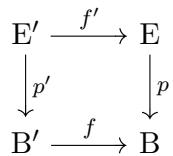
\includegraphics[keepaspectratio]{images/part001_2db9b8ac.jpg}}

a Cartesian square. Suppose that the B-space (E, p) is a covering and that the space B' is connected and locally connected. Let b' be a point of B'. For the B'-space (E', p') to be a trivializable covering, it is necessary and sufficient that for every point x of E such that \(p(x) = f(b')\) there exists a continuous lifting \(g: B' \to E\) of f such that \(g(b') = x\).

Recall that \((\mathrm{E}^{\prime}, p^{\prime})\) is a covering of \(B^{\prime}\) (I, p. 71, cor. 2) and that the map \(f^{\prime}\) induces a bijection \(E_{b^{\prime}}^{\prime} \to E_{f(b^{\prime})}\) (I, p. 10, cor.). By prop. 3 of I, p. 9, the map \(s \mapsto f^{\prime} \circ s\) defines a bijection between the set of continuous sections of \(p^{\prime}\) and the set of continuous lifts of f to E. The corollary therefore follows from Corollary 4.

PROPOSITION 7. --- Let B be a topological space, let E and E' be B-spaces, and let f: E' → E be a B-morphism. Suppose that E' is a covering of B and that the space B is locally connected.

\begin{enumerate}
\def\labelenumi{\alph{enumi})}
\item
  If the projection of the B-space E is an étale and separated map, \((\mathrm{E}^{\prime}, f)\) is a covering of E.
\item
  If f is surjective, then E is a covering of B.
\end{enumerate}

Denote by \(p\) and \(p'\) the projections of the B-spaces E and E′ respectively. Under hypothesis \(a\), \(f\) is étale (I, p. 29, prop. 6, c)). Under hypothesis \(b\), \(p\) is étale (loc. cit., d)). Consequently, under either of these two hypotheses, E is locally connected; its connected components are in particular open and closed in E (TG, I, p. 85, prop. 11).

We shall first prove Proposition 7 under the additional assumption that B is connected, locally connected, and that E' is the trivial covering (B × F', pr₁).

Lemma. --- If U is a connected component of E', the restriction of f to U induces a homeomorphism from U onto a connected component of E.

Let \(x \in F'\) such that \(U = B \times \{x\}\) (cf. I, p. 79). The map from B to E that sends \(b \in B\) to \(f(b, x)\) is a continuous section of p. Its image X is therefore connected and open in E, since p is étale (I, p. 30, cor. 3). It is moreover closed under hypothesis a), since p is separated (I, p. 27, prop. 3). It is also closed under hypothesis b) by Corollary 1 of I, p. 80, since U is open and closed in E'. Consequently, X is a connected component of E.

Since \(f \mid \mathrm{U} \colon \mathrm{U} \to \mathrm{X}\) is bijective and open, it is a homeomorphism onto its image, which proves the lemma.

Let us keep the hypotheses preceding the lemma and now prove assertion \(a\) ). Let V be a connected component of E. It is an open and closed set in E, and \(f^{-1}(\mathrm{V})\) is a union of connected components of \(\mathrm{E}'\) which \(f\) maps homeomorphically onto V by the lemma. It follows from prop. 6 of I, p. 79 that \((\mathrm{E}', f)\) is a covering.

Let us prove b). Since f is surjective, it follows from the lemma that every connected component V of E is the homeomorphic image of a connected component \(U = B \times \{x\}\) of \(E'\) . The map p then induces a homeomorphism from V onto B. By prop. 6, E is a covering of B.

This therefore proves the proposition, under the additional hypothesis that B is connected and E' is a trivializable covering of B. Let us prove it in the general case.

There exists a covering \((\mathrm{U}_{i})_{i\in\mathrm{I}}\) of B, consisting of connected open sets over which the covering \(E'\) is trivializable. Let \(i\in I\) .

Let us prove \(a\). If the map \(p\) is étale and separated, the same is true of the map \(p_{\mathrm{U}_i}\colon \mathrm{U}_i\times_{\mathrm{B}}\mathrm{E}\to \mathrm{U}_i\), for \(i\in \mathrm{I}\), by props. 8 of I, p. 31 and 4 of I, p. 27. It follows therefore from the particular case treated that, for every \(i\in \mathrm{I}\), the \(\mathrm{U}_i\)-space \((\overline{p'}^{1}(\mathrm{U}_i),f_{\mathrm{U}_i})\) is a covering. Let A denote the total space of the disjoint union \(\coprod_{i\in I}\mathrm{U}_i\) and \(q\colon \mathrm{A}\to \mathrm{B}\) the canonical map. Then, the space \(\mathrm{A}\times_{\mathrm{B}}\mathrm{E}'\), equipped with the map \(f_{\mathrm{A}}\colon \mathrm{A}\times_{\mathrm{B}}\mathrm{E}'\to \mathrm{A}\times_{\mathrm{B}}\mathrm{E}\), is a covering of \(\mathrm{A}\times_{\mathrm{B}}\mathrm{E}\). The map \(q\) admits a continuous section in a neighborhood of every point of B, and Proposition 3 of I, p. 72, applied to the Cartesian square

\[
\begin{array}{c} \mathrm {A\times_ {B} E^ {\prime}} \longrightarrow \mathrm {E^ {\prime}} \\ \Big \downarrow f _ {\mathrm{A}} \\ \mathrm {A\times_ {B} E} \longrightarrow \mathrm{E} \end{array} ,
\]

implies that \(E'\) is a covering of E.

Let us prove \(b\). Suppose that \(f\) is surjective. Then, for every element \(i\) from I, the map \(f_{\mathrm{U}_i}\colon \mathrm{U}_i\times_{\mathrm{B}}\mathrm{E}'\to \mathrm{U}_i\times_{\mathrm{B}}\mathrm{E}\) is surjective and the space \(\mathrm{U}_i\times_{\mathrm{B}}\mathrm{E}'\), equipped with the map \(f_{\mathrm{U}_i}\), is a covering of \(\mathrm{U}_i\times_{\mathrm{B}}\mathrm{E}\) (I, p. 71, cor. 2 of prop. 2). From the special case treated previously, it follows that the \(\mathrm{U}_i\)-space \((\overline{p}^{1}(\mathrm{U}_{i}),p_{\mathrm{U}_{i}})\) is a covering. Consequently, E is a covering of B.

Let B be a topological space, let E and E′ be coverings of B, and let \(f: E \rightarrow E'\) be a B-morphism. We have seen that \((E, f)\) is a covering under each of the following two hypotheses: 1) the covering E is locally of finite degree (I, p. 76, cor. 1); 2) the space B is locally connected (I, p. 81, prop. 7). This phenomenon can be explained as follows.

Let F and F′ be discrete topological spaces, and let \(f: B \times F \to B \times F'\) be a B-morphism. The map \(\widetilde{f}: b \mapsto \mathrm{pr}_{2} \circ f(b, \cdot)\) from B to the space \(\mathcal{C}_{c}(F; F')\) is continuous (TG, X, p. 28, th. 3). If U is an open subset of B such that the map \(\widetilde{f}\) is constant on U, the map \(f_{U}: U \times F \to U \times F'\) deduced from f is a trivializable covering (I, p. 69, prop. 1).

The space \(\mathcal{C}_c(\mathrm{F};\mathrm{F}')\) is none other than the set \(\mathcal{F}(\mathrm{F};\mathrm{F}')\) of maps from F into \(\mathrm{F}'\) endowed with the topology induced by the topology of the product space \((\mathrm{F}')^{\mathrm{F}}\) by the canonical identification. For this topology, the space \(\mathcal{F}(\mathrm{F};\mathrm{F}')\) is totally disconnected (I, p. 84, prop. 10). Consequently, if the space B is connected, the map \(\widetilde{f}\) is constant (I, p. 82, prop. 4); if the space B is locally connected, the map \(\widetilde{f}\) is locally constant. When the set F is finite, the space \(\mathcal{F}(\mathrm{F};\mathrm{F}')\) is discrete and the map \(\widetilde{f}\) is locally constant.

Remark. --- Let B be a topological space, let \((\mathrm{E}, p)\) and \((\mathrm{E}', p')\) be B-spaces and let \(f: E' \to E\) be a B-morphism.

\begin{enumerate}
\def\labelenumi{\alph{enumi})}
\item
  If E and E' are coverings of B, the map f is étale (I, p. 29, prop. 6) and separated (I, p. 25, prop. 2). But it is not true in general that (E', f) is a covering of E if the space B is not locally connected (I, p. 145, exerc. 4).
\item
  If \((\mathrm{E}^{\prime}, p^{\prime})\) is a covering of B, f is surjective and makes \(E^{\prime}\) a covering of E, then the map p is étale (I, p. 29, prop. 6). But it is not true, in general, that it is separated if the space B is not locally connected (I, p. 145, exerc. 4). In particular, E is not necessarily a covering of B.
\end{enumerate}

COROLLARY. --- Let B be a connected and locally connected topological space. Let E and E' be coverings of B. Let b be a point of B. Let \(f: E' \to E\) be a B-morphism and let \(f_{b}: E_{b}' \to E_{b}\) be the map induced by f by restriction to the fibers. If the map \(f_{b}\) is injective (resp. surjective, resp. bijective), then so is the map f.

Denote by \(p\) the projection of the B-space E. According to the proposition, \((\mathrm{E}', f)\) is a covering of E; its image \(f(\mathrm{E}')\) is open and closed in E. Let U denote the complement of \(f(\mathrm{E}')\) in E, so that the B-space \((\mathrm{U}, p \mid \mathrm{U})\) is a covering of B (I, p. 80, corollary 1). If the map \(f_b\) is surjective, the fiber at \(b\) of this covering is empty. Since B is a connected space, U is then empty, so \(f\) is surjective.

The set V of points of E where the fiber of f has exactly one element is open and closed. The B-spaces \((V, p|V)\) and \((f(E'), p|f(E'))\) are coverings of B (loc. cit.) and the canonical map \(i: V \to f(E')\) is a B-morphism. If the map \(f_b\) is injective, the map \(i_b\) is surjective, hence i is surjective by the preceding result, and we have \(V = f(E')\). Consequently, the map f is injective.

\subsection{Coverings of a paracompact space}

PROPOSITION 8. --- A covering of a paracompact space (I, p. 69) is a paracompact space.

Let us first prove a lemma.

Lemma. --- Let E be a separated topological space. Suppose that E has a locally finite open cover \((\mathrm{V}_{i})_{i\in\mathrm{I}}\) such that, for every \(i\in I\), \(\overline{V_{i}}\) is a paracompact space. Then the space E is paracompact.

Let \((\mathrm{W}_{j})_{j\in\mathrm{J}}\) be an open cover of E; we shall prove that there exists a locally finite open refinement \((\mathrm{A}_{k})_{k\in\mathrm{K}}\) of E which is finer than the covering \((\mathrm{W}_{j})_{j\in\mathrm{J}}\). For all \(i\in I\), let \((\mathrm{A}_{\ell}^{\prime})_{\ell\in\mathrm{K}_{i}}\) be a locally finite covering of \(\overline{V_{i}}\) by open subsets of \(\overline{V_{i}}\), finer than the covering \((\mathrm{W}_{j}\cap\overline{\mathrm{V}_{i}})_{j\in\mathrm{J}}\). Let K be the sum of the family \((\mathrm{K}_{i})_{i\in\mathrm{I}}\) (E, II, p. 30, def. 8). For every element \(k=(\ell,i)\) of K, set \(A_{k}=A_{\ell}^{\prime}\cap V_{i}\). Then \(A_{k}\) is open in E and one has \(\bigcup_{k\in K}A_{k}=\bigcup_{i\in I}V_{i}=E\); moreover, for every \(k\in K\), there exists an index \(j\in J\) such that \(A_{k}\subset W_{j}\). Thus, the family \((\mathrm{A}_{k})_{k\in\mathrm{K}}\) is an open cover of E finer than \((\mathrm{W}_{j})_{j\in\mathrm{J}}\). It remains to prove that the family \((\mathrm{A}_{k})_{k\in\mathrm{K}}\) is locally finite. Let \(x\in E\); there exists an open neighborhood U of x that meets \(V_{i}\) only for i belonging to a finite subset I' of I. For every \(i\in I'\), x has an open neighborhood \(U_{i}\subset U\) that meets only finitely many open sets \(A_{k}\), for \(k\in K_{i}\times\{i\}\): this is obvious if x does not belong to \(\overline{V_{i}}\), and if x belongs to \(\overline{V_{i}}\), this follows from the local finiteness property of the covering \((\mathrm{A}_{\ell}^{\prime})_{\ell\in\mathrm{K}_{i}}\) of \(\overline{V_{i}}\). Consequently, \(V^{\prime}=\bigcap_{i\in I'}U_{i}\) is an open neighborhood of x that meets only finitely many of the \(A_{k}\), \(k\in K\), and the covering \((\mathrm{A}_{k})_{k\in\mathrm{K}}\) is locally finite.

Let us prove the proposition. Let E be a covering of B, denote its projection by p, and suppose that the space B is paracompact. Let \((\mathrm{A}_{i})_{i\in\mathrm{I}}\) be a locally finite open cover of B such that, for every \(i\in I\), the covering E is trivializable over \(A_{i}\). For all \(i\in I\), let \(F_{i}\) be a discrete topological space and let \(g_{i}\colon\overline{p}^{1}(\mathrm{A}_{i})\to\mathrm{A}_{i}\times\mathrm{F}_{i}\) be a trivialization of E over \(A_{i}\). Let \((\mathrm{B}_{i})_{i\in\mathrm{I}}\) be an open cover of B such that, for every \(i\in I\), one has \(\overline{B_{i}}\subset A_{i}\) (TG, IX, p. 49, prop. 4 and p. 48, cor. 1). For every \(i\in I\), set \(V_{i}=\overline{p}^{1}(\mathrm{B}_{i})\); we have \(\overline{V_{i}}\subset\overline{p}^{1}(\overline{\mathrm{B}_{i}})\subset\overline{p}^{1}(\mathrm{A}_{i})\) and \(V_{i}=\overline{g_{i}}^{1}(\mathrm{B}_{i}\times\mathrm{F}_{i})\), whence \(\overline{V_{i}}\subset\overline{g_{i}}^{1}(\overline{\mathrm{B}_{i}}\times\mathrm{F}_{i})\). Since B is paracompact, \(\overline{B_{i}}\) is paracompact (TG, I, p. 69, prop. 16) and \(\overline{B_{i}}\times F_{i}\) is paracompact (TG, I, p. 70, prop. 18). Consequently, \(\overline{g_{i}}^{1}(\overline{\mathrm{B}_{i}}\times\mathrm{F}_{i})\) is paracompact, hence \(\overline{V_{i}}\) also (TG, I, p. 69, prop. 16). The family \((\mathrm{V}_{i})_{i\in\mathrm{I}}\) is, by construction, a locally finite open covering of E. Finally, the space E is separated (I, p. 26, remark 3). It therefore satisfies the hypotheses of the lemma, whence the proposition.

Remark. --- One can show that a covering of a metrizable space is metrizable (I, p. 145, exerc. 1) and that a connected covering of a locally compact, countable-at-infinity space is itself locally compact and countable at infinity (I, p. 145, exerc. 2).

\subsection{Locally constant sheaves}

Let B be a topological space and F a set; endow F with the discrete topology. One calls the constant sheaf on B with stalk-type F the sheaf on B of locally constant functions with values in F (I, p. 45, example 2). This sheaf is sometimes denoted \(\underline{\mathbf{F}}\), when no confusion about the space B is to be feared. It is identified with the sheaf on B of continuous sections of the étale B-space \((B \times F,\mathrm{pr}_1)\): the formula \(i([U,s,a]) = (a,s(a))\) indeed defines a canonical isomorphism \(i\) from the étalé space associated with \(\underline{\mathbf{F}}\) onto \((B \times F,\mathrm{pr}_1)\). For every \(a \in B\), the map \([U,s,a] \mapsto s(a)\) is a canonical bijection of the stalk \(\underline{\mathbf{F}}_a\) of \(\underline{\mathbf{F}}\) at \(a\) onto the set F.

Let \(\mathcal{P} = (\mathcal{P}(\mathrm{U}), r_{\mathrm{UV}})\) be the presheaf on B such that \(\mathcal{P}(\mathrm{U}) = \mathrm{F}\) for every open set U of B and \(r_{\mathrm{UV}} = \mathrm{Id}_{\mathrm{F}}\) for every pair (U, V) of open sets of B such that \(\mathrm{U} \subset \mathrm{V}\). Then, the sheaf \(\widetilde{\mathcal{P}}\) associated with \(\mathcal{P}\) is canonically isomorphic to the constant sheaf \(\underline{\mathrm{F}}\) (I, p. 52, example 1).

DEFINITION 3. --- A sheaf \(\mathcal{F}\) on a topological space B is locally constant if every point of B has an open neighborhood U such that the induced sheaf \(\mathcal{F} \mid U\) is isomorphic to a constant sheaf on U.

PROPOSITION 9. --- For a sheaf to be locally constant, it is necessary and sufficient that the associated étalé space be a covering.

Let B be a topological space and let \(\mathcal{F}\) be a sheaf on B. The sheaf \(\mathcal{F}\) is constant if and only if the étalé space \(\mathrm{E}_{\mathcal{F}}\) is B-isomorphic to a trivial covering \((\mathrm{B} \times \mathrm{F},\mathrm{pr}_1)\), where F is a discrete topological space. If U is an open subset of B, the étalé space associated with the induced sheaf \(\mathcal{F} \mid \mathrm{U}\) is identified with the U-étale space induced by \(\mathrm{E}_{\mathcal{F}}\) above U (cf. I, p. 51). The proposition follows from this.

COROLLARY. --- For an étale B-space to be a covering, it is necessary and sufficient that the sheaf of its sections be locally constant.

This follows from the proposition and from Example 2 of I, p. 52.

\subsection{Products of locally constant sheaves}

Let B be a topological space and let \((\mathcal{F}_{i})_{i\in\mathrm{I}}\) be a family of sheaves on B. Denote by \(\mathcal{F}\) the product sheaf \(\prod_{i\in I}\mathcal{F}_{i}\) and, for \(i\in I\), let \(pr_{i}\colon \mathcal{F}\to\mathcal{F}_{i}\) be the projection morphism of index i (I, p. 46, example 7). Let \((\mathrm{E},p)\) and \((\mathrm{E}_{i},p_{i})\) be the étalé B-spaces associated with the sheaves \(\mathcal{F}\) and \(\mathcal{F}_{i}\), respectively, and let \(\varphi_{i}\colon \mathrm{E}\to \mathrm{E}_{i}\) be the B-morphism associated with \(pr_{i}\) (I, p. 50). Finally, let us denote by \((\mathrm{E}^{\prime},p^{\prime})\) the B-product \(\prod_{B}\mathrm{E}_{i}\). By the universal property of the B-space product (I, p. 5), there exists a unique B-morphism \(\Phi\colon \mathrm{E}\to \mathrm{E}^{\prime}\) such that, for every \(i\in I\), \(pr_{i}\circ\Phi=\varphi_{i}\).

PROPOSITION 10. --- If the set I is finite, the B-morphism \(\Phi\) is an isomorphism.

By the corollary of I, p. 32, the B-space \(\mathrm{E}'\) is étale, and it suffices to show that the B-morphism \(\Phi\) is bijective (I, p. 30, cor. 2). For every point b of B, the restriction \(\Phi_b\colon \mathrm{E}_b\to \mathrm{E}'_b\) of \(\Phi\) to the fibers at b is identified with the canonical map from \(\varinjlim\prod_{i\in I}\mathcal{F}_{i}(U)\) to \(\prod_{i\in I}\varinjlim\mathcal{F}_{i}(U)\), where U ranges over the open subsets of B containing b (cf. I, p. 50). By prop. 10 of E, III, p. 67, this map is a bijection.

Now consider the case of locally constant sheaves on a topological space B. Let \((\mathrm{F}_{i})_{i\in\mathrm{I}}\) be a family of sets and set \(F=\prod_{i\in I}F_{i}\) . One defines a canonical morphism \(\psi=(\psi_{\mathrm{U}})\) from the constant sheaf \(\underline{F}\) into the product \(\prod_{i\in I}\underline{F}_{i}\) of the constant sheaves \(\underline{F}_{i}\) by setting, for every open subset U of B and every locally constant function \(f\colon U\to F\) , \(\psi_{\mathrm{U}}(f)=(\mathrm{pr}_{i}\circ f)_{i\in\mathrm{I}}\) .

PROPOSITION 11. --- If the set I is finite, or if the space B is locally connected, the canonical morphism \(\psi\colon\underline{\mathbf{F}}\to\prod\underline{\mathbf{F}_{i}}\) is an isomorphism.

Let U be an open subset of B. It is clear that the map \(\psi_{\mathrm{U}}\) is injective. Let us show that it is surjective. It suffices to prove that for every family \((f_i)_{i\in \mathrm{I}}\) where \(f_{i}\) is a locally constant map from U into \(\mathrm{F}_i\), and every point \(a\) of U, there exists a neighborhood V of \(a\) in U such that for every \(i\in \mathrm{I}\), the map \(f_{i}|\mathrm{V}\) is constant. When the set I is finite, the existence of such a neighborhood is clear. When the space B is locally connected, it suffices to take for V a connected neighborhood of \(a\) in U. This proves the proposition.

COROLLARY 1. --- A finite product of locally constant sheaves is locally constant.

Let \((\mathcal{F}_{i})_{i\in\mathrm{I}}\) be a finite family of locally constant sheaves on B. Every point a of B has an open neighborhood U in B such that, for every \(i\in I\), the sheaf \(\mathcal{F}_{i}\mid U\) is isomorphic to a constant sheaf. The same is then true of the sheaf \((\prod\mathcal{F}_{i})\mid U\), which is equal to \(\prod(\mathcal{F}_{i}\mid U)\).

COROLLARY 2. --- Let \((\mathcal{F}_{i})_{i\in I}\) be a family of sheaves on B. Suppose that the space B is locally connected and that every point of B has an open neighborhood U such that, for every \(i\in I\) , the sheaf \(\mathcal{F}_{i}|U\) is isomorphic to a constant sheaf. Then, the product sheaf \(\prod \mathcal{F}_{i}\) is locally constant.

Remarks. --- 1) Let \((\mathrm{E}_{i}, p_{i})_{i \in \mathrm{I}}\) be a family of coverings of the topological space B. Suppose that the space B is locally connected and that there exists an open covering \((\mathrm{U}_{j})_{j \in \mathrm{J}}\) of B such that, for every \(j \in J\) and every \(i \in I\) the covering \(E_{i}\) is trivializable over \(U_{j}\) . For \(i \in I\), let \(F_{i}\) be the locally constant sheaf of sections of \(E_{i}\) and let \(F\) be the product sheaf \(\prod_{i} F_{i}\) . By the preceding corollary, F is a locally constant sheaf and the étale B-space E associated with it is therefore a covering (I, p. 86, prop. 8). For \(i \in I\), let \(pr_{i}: E \to E_{i}\) be the B-morphism induced by the projection morphism of index i, \(F \to F_{i}\) .

Now consider a covering (Y, q) of B and, for every \(i \in I\), let \(f_i \colon Y \to E_i\) be a B-morphism. If G denotes the locally constant sheaf of sections of q, the B-morphisms \(f_i\) induce sheaf morphisms \(\widetilde{f}_i \colon G \to F_i\) . Let \(\widetilde{f} \colon G \to F\) be the unique morphism of sheaves such that \(\widetilde{f}_i = pr_i \circ \widetilde{f}\) for all \(i \in I\) . There then exists a unique B-morphism \(f \colon Y \to E\) such that \(f_i = pr_i \circ f\) for every i: it is the B-morphism which induces \(\widetilde{f}\) .

One sometimes says that E is the product covering of the family \((\mathrm{E}_i)_{i\in \mathrm{I}}\).

\begin{enumerate}
\def\labelenumi{\arabic{enumi})}
\setcounter{enumi}{1}
\tightlist
\item
  With the preceding notations, the canonical B-morphism \(\Phi\colon\mathrm{E}\to\Pi_{\mathrm{B}}\mathrm{E}_{i}\) is bijective. The question is indeed local in nature on B, and one may suppose that, for every \(i\in\mathrm{I}\), the B-space \(\mathrm{E}_{i}\) is isomorphic to the B-space \((\mathrm{B}\times\mathrm{F}_{i},\mathrm{pr}_{1})\), where \(\mathrm{F}_{i}\) is a discrete topological space, so that the sheaf \(\mathcal{F}_{i}\) is isomorphic to the sheaf \(\underline{\mathrm{F}}_{i}\). By prop. 11, the sheaf \(\mathcal{F}\) is identified with the sheaf \(\underline{\mathrm{F}}\), where \(\mathrm{F}\) is the set \(\prod\mathrm{F}_{i}\), endowed with the discrete topology, and the map \(\Phi\) is identified with the canonical map \(B \times F \rightarrow B \times (\prod_{i} F_{i})\) which is bijective.
\end{enumerate}

\subsection{Morphisms of locally constant sheaves on a locally connected space}

Let B be a topological space, let \((\mathrm{E},p)\) and \((\mathrm{E}^{\prime},p^{\prime})\) be B-spaces. Denote by \(\mathcal{M} = \underline{\mathcal{M}or_{\mathrm{B}}(\mathrm{E};\mathrm{E}^{\prime})}\) the sheaf on B of B-morphisms from \((\mathrm{E},p)\) to \((\mathrm{E}^{\prime},p^{\prime})\) (I, p. 45, example 4). If U is an open set of B and b a point of U, we denote by \(\theta_{b,\mathrm{U}}\colon\mathcal{M}(\mathrm{U})\to\mathcal{C}(\mathrm{E}_{b};\mathrm{E}_{b}^{\prime})\) the canonical map obtained by passing to fibers at b. We denote by \(\theta_{b}\colon\mathcal{M}_{b}\to\mathcal{C}(\mathrm{E}_{b};\mathrm{E}_{b}^{\prime})\) the unique map such that \(\theta_{b,\mathrm{U}}\) is the composite of \(\theta_{b}\) and the canonical map \(\mathcal{M}(\mathrm{U})\to\mathcal{M}_{b}\) for every open set U of B containing b (E, III, p. 62).

Let also \(\mathcal{I} = \underline{\mathcal{I}som}_{\mathrm{B}}(\mathrm{E};\mathrm{E}^{\prime})\) be the sheaf on B of B-isomorphisms from \((\mathrm{E},p)\) to \((\mathrm{E}^{\prime},p^{\prime})\). Denote by \(i\colon \mathcal{I}\to \mathcal{M}\) the canonical morphism. For every \(b\in \mathrm{B}\), the map \(\theta_{b}\circ i_{b}\) induces a map \(\theta_b^\prime\) of \(\mathcal{I}_b\) into the set of continuous bijections of \(\mathrm{E}_b\) onto \(\mathrm{E}_b^\prime\).

PROPOSITION 12. --- Suppose that the space B is locally connected and that the B-spaces E and E' are coverings. The sheaf \(\mathcal{M}or_{\mathrm{B}}(\mathrm{E};\mathrm{E}')\) is then locally constant and, for every \(b\in\mathrm{B}\), the map \(\theta_{b}\) is a bijection from its stalk at \(b\) onto the set of maps from \(\mathrm{E}_{b}\) to \(\mathrm{E}_{b}^{\prime}\).

Similarly, the sheaf \(\mathcal{I}\text{som}_{\mathrm{B}}(\mathrm{E};\mathrm{E}^{\prime})\) is locally constant and, for every point \(b\) of B, the map \(\theta_{b}^{\prime}\) is a bijection from its stalk at \(b\) onto the set of bijections of \(\mathrm{E}_{b}\) onto \(\mathrm{E}_{b}^{\prime}\).

We shall denote by \(\mathcal{M} = \underline{\mathcal{M}or}_{\mathrm{B}}(\mathrm{E};\mathrm{E}^{\prime})\) and \(\mathcal{I} = \underline{\mathcal{Isom}}_{\mathrm{B}}(\mathrm{E};\mathrm{E}^{\prime})\). The assertions to be proved are local in nature on B; we may therefore assume that \(\mathrm{E} = \mathrm{B}\times \mathrm{F}\) and \(\mathrm{E}' = \mathrm{B}\times \mathrm{F}'\) are trivial coverings, where F and \(\mathrm{F}'\) are discrete topological spaces.

First, let us prove that, for every connected open subset U of B and every point b of U, the map \(\theta_{b,U}\) is a bijection. Let \(f\colon U\times F\to U\times F'\) be a morphism of U-spaces; then, \(\theta_{b,U}(f)\) is the map \(y\mapsto\mathrm{pr}_{2}(f(b,y))\) from F to \(F'\). For all \(y\in F\), the map \(x\mapsto\mathrm{pr}_{2}(f(x,y))\) is a continuous map from the connected space U into the discrete space \(F'\), hence is constant, equal to \(\mathrm{pr}_{2}(f(b,y))\). One thus has \(f(x,y)=(x,\theta_{b,U}(f)(y))\). It follows that \(\theta_{b,U}\) is a bijection;

its inverse bijection associates to every map \(\varphi\colon\mathrm{F}\to\mathrm{F}^{\prime}\) the U-morphism from \(\mathrm{U}\times\mathrm{F}\) to \(\mathrm{U}\times\mathrm{F}^{\prime}\) given by \((x,y)\mapsto(x,\varphi(y))\).

By hypothesis, every point \(b \in B\) admits a base of connected open neighborhoods; the map \(\theta_{b}\) is therefore a bijection. The maps \(\theta_{b,\mathrm{U}}^{-1}\), for U a nonempty connected open subset of B and b an arbitrary point of B, define a morphism of presheaves (with respect to the base of connected open subsets of B) from the constant sheaf with stalk-type \(F^{\prime F}\) to the sheaf \(\mathcal{M}\). By what precedes, this morphism induces a bijection on stalks; it is therefore an isomorphism.

The assertions concerning the sheaf \(\mathcal{I}\) are proved similarly.

COROLLARY 1. --- Let B be a topological space and A a subspace of B. Suppose that the spaces A and B are locally connected. Let E and E' be coverings of B. Then the canonical morphisms \(\psi\colon\mathcal{M}or_{B}(E;E')_{A}\to\mathcal{M}or_{A}(E_{A};E'_{A})\) and \(\psi'\colon\mathcal{I}som_{B}(E;E')_{A}\to\mathcal{I}som_{A}(E_{A};E'_{A})\) (I, p. 45, example 4) are isomorphisms.

For every point \(a \in \mathrm{A}\), it follows from the preceding proposition and from example 2 of I, p. 63, applied to the spaces \(\{a\}\), A, B and to the canonical injections, that the canonical morphism \(\psi\) induces, by passage to stalks, the identity on \(\mathrm{E}_a^{\mathrm{E}_a'}\). It is therefore an isomorphism. The fact that \(\psi'\) is an isomorphism is proved in an analogous manner.

COROLLARY 2. --- Let B be a topological space and A a subspace of B. Suppose that the spaces A and B are locally connected and that the pair (B, A) has property (PCV) of I, p. 37. Let E and E' be coverings of B, and denote their projections by p and p'. Let \(g: \overline{p}^{1}(A) \to (\overline{p}')^{1}(A)\) be an A-morphism (resp. an A-isomorphism). There exists a neighborhood U of A in B and a U-morphism (resp. a U-isomorphism) \(f: \overline{p}^{1}(U) \to (\overline{p}')^{1}(U)\) such that \(f_{A} = g\).

Let us keep the notation of Corollary 1. By that same corollary, an A-morphism \(g \colon \mathrm{E}_{\mathrm{A}} \to \mathrm{E}_{\mathrm{A}}^{\prime}\) is identified with a section \(s_0\) over A of the étale space \(\mathrm{E}_{\mathcal{M}}\) associated with \(\mathcal{M}\). By the hypothesis made on the pair (B, A) and Lemma 3 of I, p. 39, there exists an open neighborhood U of A in B and a continuous section \(s\) of \(\mathrm{E}_{\mathcal{M}}\) above U extending \(s_0\). This section \(s\) is identified with a U-morphism \(f \colon \mathrm{E}_{\mathrm{U}} \to \mathrm{E}_{\mathrm{U}}^{\prime}\) extending \(g\).

The case where g is an A-isomorphism is handled analogously by considering, in place of the sheaf M, the sheaf S.

\section{PRINCIPAL COVERINGS}

\subsection{Principal fiber bundles}

DEFINITION 1. --- Let G be a topological group and B a topological space. A (right) principal fiber bundle with base B and group G is a B-space (E, p) equipped with a right action of G on E (A, I, p. 50) having the following property:

(FP) For every point \(b\) of \(B\), there exists a neighborhood \(U\) of \(b\) and a U-isomorphism \(f\colon U\times G\to \overline{p}^{1}(U)\) such that for all \(u\in U\) and \(g,g'\in G\), one has \(f(u,gg')=f(u,g)\cdot g'\).

Instead of saying that \((E, p)\) is a principal fiber bundle with base B and group G, one sometimes says that the quadruple \((E, G, B, p)\) is a principal fibration (cf. VAR, R, §6), or by abuse of language that the map \(p: E \to B\) is a principal fibration with base B and group G.

When no doubt is possible as to the base B, the group G, and the action of G on E, we will simply say that \((E, p)\) is a principal fiber bundle.

Let G be a topological group. Let \((E,p)\) be a B-space equipped with a left action of G. If, for the right action of the group \(G^{\circ}\), opposite to the given operation (A, I, p. 50), \((E,p)\) is a principal right fiber bundle with group \(G^{\circ}\), we say that \((E,p)\) is a principal left fiber bundle with group G.

A principal fiber bundle is a locally trivial fiber bundle (I, p. 68, def. 1).

It follows from property (FP) that the group G acts continuously (TG, III, p. 9) and freely on E, and that the orbits of this action are the fibers of the B-space (E, p). The map \(p' \colon \mathrm{E} / \mathrm{G} \to \mathrm{B}\) deduced from \(p\) is continuous and bijective. Again by property (FP), the map \(p\) is open (TG, I, p. 30, prop. 2 and p. 26, prop. 5); consequently, \(p'\) is a homeomorphism (TG, I, p. 32, prop. 3).

Let \((\mathrm{E},p)\) and \((\mathrm{E}^{\prime},p^{\prime})\) be principal fiber bundles with base B and group G. We say that a map \(f: E \to E^{\prime}\) is a morphism of principal fiber bundles (with base B and group G) if f is a B-morphism and one has \(f(x \cdot g) = f(x) \cdot g\) for all \(x \in E\) and every \(g \in G\). Let \((\mathrm{E}^{\prime\prime},p^{\prime\prime})\) be a principal fiber bundle with base B and group G. If \(f: \mathrm{E} \to \mathrm{E}'\) and \(g: \mathrm{E}' \to \mathrm{E}''\) are morphisms of principal fiber bundles, the map \(g \circ f: \mathrm{E} \to \mathrm{E}''\) is a morphism of principal fiber bundles. In accordance with the general definitions (E, IV, p. 11), one may take as morphisms of the principal fiber-bundle structure with base B and group G those defined above. We denote \(\mathcal{C}_{\mathrm{B}}^{\mathrm{G}}(\mathrm{E}; \mathrm{E}')\) the set of morphisms of principal fiber bundles from \((\mathrm{E}, p)\) to \((\mathrm{E}',p')\).

We call the trivial principal fiber bundle with base B and group G the B-space \((B \times G, pr_{1})\) endowed with the right action of G on \(B \times G\) defined by \((b, g) \cdot h = (b, gh)\) .

A principal fiber bundle (E, p) with base B and group G is said to be trivializable if there exists an isomorphism from (E, p) onto the trivial principal fiber bundle \((B \times G,\mathrm{pr}_{1})\); such an isomorphism is called a trivialization of the principal fiber bundle (E, p). Property (FP) expresses that there exists an open covering \((\mathrm{U}_{i})_{i \in \mathrm{I}}\) of B such that, for every \(i \in I\), the \(\mathrm{U}_{i}\)-space \((\overline{p}^{1}(\mathrm{U}_{i}), p \mid \mathrm{U}_{i})\), endowed with the right action of G induced by that of G on E, is a trivializable principal fiber bundle.

Examples. --- 1) Let (E, p) be a principal fiber bundle with base B and group G, and let A be a subspace of B. The subspace \(E_{A} = \overline{p}^{1}(A)\) of E is stable under the action of G, and the map \(p_{A}: E_{A} \to A\) makes it a principal fiber bundle with base A and group G. One says that \((E_{A}, p_{A})\) is the principal fiber bundle induced by (E, p) over A.

\begin{enumerate}
\def\labelenumi{\arabic{enumi})}
\setcounter{enumi}{1}
\tightlist
\item
  Let (E, p) be a principal fiber bundle with base B and group G; let \((\mathrm{E}^{\prime}, p^{\prime})\) be a principal fiber bundle with base \(B^{\prime}\) and group \(G^{\prime}\). One defines a right action of the group \(G \times G^{\prime}\) on the space \(E \times E^{\prime}\) by setting \((x, x^{\prime}) \cdot (g, g^{\prime}) = (x \cdot g, x^{\prime} \cdot g^{\prime})\) for \(x \in E\), \(x^{\prime} \in E^{\prime}\), \(g \in G\) and \(g^{\prime} \in G^{\prime}\); this action is continuous. Let U be an open subset of B and \(f: U \times G \to \overline{p}^{1}(U)\) a trivialization of the U-space \((\overline{p}^{1}(U), p_{\mathrm{U}})\); let \(U^{\prime}\) be an open subset of \(B^{\prime}\) and \(f^{\prime}: U^{\prime} \times G^{\prime} \to \overline{p'}^{1}(U^{\prime})\) a trivialization of the \(U^{\prime}\)-space \((\overline{p'}^{1}(U^{\prime}), p_{\mathrm{U}}^{\prime})\). The map \(((b, b^{\prime}), (g, g^{\prime})) \mapsto (f(b, g), f'(b', g'))\) is a \((\mathrm{U} \times \mathrm{U}^{\prime})\)-isomorphism \(f''\) of \((\mathrm{U} \times \mathrm{U}^{\prime}) \times (\mathrm{G} \times \mathrm{G}^{\prime})\) onto \(\overline{p}^{1}(U) \times \overline{p'}^{1}(U^{\prime})\) and one has
\end{enumerate}

\[
f ^ {\prime \prime} ((b, b ^ {\prime}), (g h, g ^ {\prime} h ^ {\prime})) = (f (b, g h), f ^ {\prime} (b ^ {\prime}, g ^ {\prime} h ^ {\prime})) = f ^ {\prime \prime} ((b, b ^ {\prime}), (g, g ^ {\prime})) \cdot (h, h ^ {\prime}).
\]

It follows that the \((\mathrm{B} \times \mathrm{B}')\)-space \(E \times E'\), endowed with the action of \(G \times G'\) defined above, is a principal fiber bundle, called the product of the principal fiber bundles E and E'.

\begin{enumerate}
\def\labelenumi{\arabic{enumi})}
\setcounter{enumi}{2}
\item
  In particular, when \(B = B'\) , the B-space \(E \times_{B} E'\) is identified with the principal fiber bundle with group \(G \times G'\) induced by \(E \times E'\) over the diagonal \(\Delta_{B}\) of \(B \times B\) . Endowed with this principal fiber bundle structure, the B-space \(E \times_{B} E'\) is called the fibered product of the principal fiber bundles E and \(E'\) .
\item
  Let E be a principal fiber bundle with base B and group G, and let F be a topological space. The \((B \times F)\) -space \(E \times F\) endowed with the action \((x, y) \cdot g = (x \cdot g, y)\) , for \(x \in E\) , \(y \in F\) and \(g \in G\) , is a principal fiber bundle with group G. This is the particular case of Example 2, where \(p'\) is the identity map of F and \(G'\) is a group reduced to the identity element.
\item
  Let B be a topological space and (E, p) a principal fiber bundle with base B and group G. Let B' be a topological space and \(f: B' \to B\) a continuous map. The group G acts on the right on the fibered product \(B' \times_{B} E\) by the law \((b', x) \cdot g = (b', x \cdot g)\) , for \(b' \in B'\) , \(x \in E\) and \(g \in G\) . This action is continuous and free; the orbits are the fibers of the map \(pr_{1}: B' \times_{B} E \to B'\) . It follows from Examples 1 and 4 above and from Remark 2 of I, p. 16 that the \(B'\) -space \(B' \times_{B} E\) is a principal fiber bundle with group G. It is called the principal fiber bundle deduced from (E, p) by the base change f, or also the inverse image of (E, p) under f.
\end{enumerate}

PROPOSITION 1. --- Every morphism of principal fiber bundles is an isomorphism.

Let \(f \colon \mathrm{B} \times \mathrm{G} \to \mathrm{B} \times \mathrm{G}\) be a morphism of the trivial principal fiber bundle \((\mathrm{B} \times \mathrm{G},\mathrm{pr}_1)\) into itself and let \(\varphi \colon \mathrm{B} \times \mathrm{G} \to \mathrm{G}\) be the continuous map \(\mathrm{pr}_2 \circ f\), such that \(f(b, g) = (b, \varphi(b, g))\). For all \(b \in \mathrm{B}\) and all \(g, h \in \mathrm{G}\), we have \(\varphi(b, gh) = \varphi(b, g) \cdot h\), whence \(\varphi(b, g) = \varphi(b, e) \cdot g\), where \(e\) denotes the identity element of \(\mathrm{G}\). The morphism \(f\) is therefore an isomorphism whose inverse morphism \(f^{-1}\) is defined by \(f^{-1}(b, g) = (b, \varphi(b, e)^{-1}g)\) for \((b, g) \in \mathrm{B} \times \mathrm{G}\).

Now let E and \(E'\) be principal fiber bundles and let \(f: E \to E'\) be a morphism of principal fiber bundles. Given property (FP), for every point \(b \in B\) there exists an open neighborhood U of b such that the principal bundles \(E_{U}\) and \(E'_{U}\) are trivializable.

By passing to subspaces, \(f\) induces a morphism \(f_{\mathrm{U}}: \mathrm{E}_{\mathrm{U}} \to \mathrm{E}_{\mathrm{U}}'\) of principal fiber bundles; according to the preceding, this morphism \(f_{\mathrm{U}}\) is an isomorphism. In particular, \(f_{b}: \mathrm{E}_{b} \to \mathrm{E}_{b}'\) is a bijection. There then exists a unique map \(g: \mathrm{E}' \to \mathrm{E}\) that induces the bijection \(f_{b}^{-1}\) by passing to subspaces. According to Proposition 4 of I, p. 19, the map \(g\) is continuous; therefore \(f\) is an isomorphism of principal fiber bundles.

COROLLARY. --- Let G be a topological group, \((E, p)\) and \((E', p')\) be principal fiber bundles with group G and bases B and B' respectively. Let \(f: B' \to B\) and \(f': E' \to E\) be continuous maps such that \(p \circ f' = f \circ p'\) and such that, for every \(x' \in E'\) and every \(g \in G\), \(f'(x' \cdot g) = f'(x') \cdot g\). Then the square

\pandocbounded{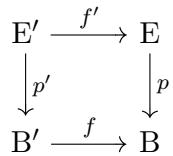
\includegraphics[keepaspectratio]{images/part001_eb35a58e.jpg}}

is a Cartesian square.

Indeed, the map \(h: E' \to B' \times_{B} E\) defined by \(h(x') = (p'(x'), f'(x'))\) is a \(B'\)-morphism of principal fiber bundles, hence an isomorphism; moreover, we have \(pr_{2} \circ h = f'\), whence the result (I, p. 8, prop. 2).

Under the hypotheses of the preceding corollary, one sometimes says that \(f'\) is an f-morphism of principal fiber bundles.

PROPOSITION 2. --- Let (E, p) be a principal fiber bundle with base B and group G, and let \(\varepsilon\) be the section \(b \mapsto (b, e)\) of the trivial principal fiber bundle (B \(\times\) G, \(\mathrm{pr}_{1}\)), where \(e\) denotes the identity element of G. The map \(h \mapsto h \circ \varepsilon\) is a bijection from \(\mathcal{C}_{\mathrm{B}}^{\mathrm{G}}(\mathrm{B} \times \mathrm{G}; \mathrm{E})\) onto the set \(\mathcal{S}(\mathrm{B}; \mathrm{E})\) of continuous sections of \(p\). The inverse bijection associates to a continuous section \(s\) of \(p\) the B-morphism \((b, g) \mapsto s(b) \cdot g\).

COROLLARY. --- A principal fiber bundle is trivializable if and only if it admits a continuous section.

PROPOSITION 3. --- Let E and B be topological spaces, \(p\colon\mathrm{E}\to\mathrm{B}\) a continuous map and G a topological group acting on the right on E. The following conditions are equivalent:

\begin{enumerate}
\def\labelenumi{(\roman{enumi})}
\item
  Endowed with the map p, E is a principal fiber bundle with base B and group G;
\item
  For every \(x \in E\) and every \(g \in G\) , we have \(p(x \cdot g) = p(x)\) , the map \(\theta: (x, g) \mapsto (x, x \cdot g)\) is a homeomorphism of \(E \times G\) onto \(E \times_{B} E\) and every point of B has a neighborhood on which there exists a continuous section of the map p.
\end{enumerate}

(i)⇒(ii): Suppose that (E, p) is a principal fiber bundle. The group G acts continuously and freely on E with the fibers of p as orbits. Consequently, the map \(\theta\) is bijective and continuous. More precisely, if one equips \(E \times_{B} E\) with the action of G defined by \((x, y) \cdot g = (x, y \cdot g)\), the map \(\theta\) is an E-morphism of the trivial principal fiber bundle \(E \times G\) into the principal fiber bundle \((E \times_{B} E \to E, \mathrm{pr}_{1})\) (Example 5), hence an isomorphism (Proposition 1). The other assertions of (ii) follow immediately from the definition.

(ii)⇒(i): Set \(\varphi = pr_{2} \circ \theta^{-1}\) , so that, for every \((x, y) \in E \times_{B} E\) , we have

\[
\theta^ {- 1} (x, y) = (x, \varphi (x, y)).\tag{1}
\]

The map \(\varphi\colon\mathrm{E}\times_{\mathrm{B}}\mathrm{E}\to\mathrm{G}\) is continuous and, for \((x,y)\in\mathrm{E}\times_{\mathrm{B}}\mathrm{E}\), the element \(\varphi(x,y)\) is the unique element \(g\) of G such that \(y=x\cdot g\). Let \(b\) be a point of B; let U be a neighborhood of \(b\) and let \(s\) be a continuous section of \(p\) above U. For \((u,g)\in\mathrm{U}\times\mathrm{G}\), set \(f(u,g)=s(u)\cdot g\); the map \(f\) is a U-morphism from \(U \times G\) to \(\overline{p}^{-1}(\mathrm{U})\). For \(y\in\overline{p}^{-1}(\mathrm{U})\), set \(f'(y)=(p(y),\varphi(s(p(y)),y))\). The map \(f'\) is a U-morphism from \(\overline{p}^{-1}(\mathrm{U})\) to U \(\times\) G. We have

\[
(f \circ f ^ {\prime}) (y) = s (p (y)) \cdot \varphi (s (p (y)), y) = y.
\]

On the other hand, for \((u,g)\in \mathrm{U}\times \mathrm{G}\) , we have

\[
(f ^ {\prime} \circ f) (u, g) = f ^ {\prime} (s (u) \cdot g) = (u, \varphi (s (u), s (u) \cdot g)) = (u, g).
\]

Therefore, f is a U-isomorphism. It follows that \((E,p)\) is a principal fiber bundle with base B and group G.

Remark 1. --- Let (E, p) be a principal fiber bundle with base B and group G. With the notation of Proposition 3, the map \(\theta^{-1}\colon E \times_{B} E \to E \times G\) is a trivialization of the principal fiber bundle \(\mathrm{pr}_{1}\colon E \times_{B} E \to E\). One says that \(\theta^{-1}\) is the canonical trivialization of this principal fiber bundle.

COROLLARY 1. --- Let G be a topological group acting continuously on the right on a topological space E. The following conditions are equivalent:

\begin{enumerate}
\def\labelenumi{(\roman{enumi})}
\item
  The orbit space E/G is Hausdorff, and the space E, equipped with the canonical map \(p: E \rightarrow E/G\), is a principal fiber bundle with group G;
\item
  The group G acts properly (TG, III, p. 27) and freely on E, and every point of E/G has a neighborhood on which there exists a continuous section of the map p.
\end{enumerate}

Set \(B=E/G\). Under each of the hypotheses (i) and (ii), the group G acts continuously and freely on E, so that the map \(\theta\colon(x,g)\mapsto(x,x\cdot g)\) is a continuous bijection from \(E\times G\) onto \(E\times_{B}E\). Let us place ourselves under this hypothesis and denote by \(\varphi\colon E\times_{B}E\to G\) the map \(pr_{2}\circ\theta^{-1}\). Taking formula (1) into account, for \(\theta\) to be a homeomorphism, it is necessary and sufficient that the map \(\varphi\) be continuous. On the other hand, since the equivalence relation defined by G is open (TG, III, p. 10, lemma 2), for the space E/G to be Hausdorff, it is necessary and sufficient that the graph \(E\times_{B}E\) of this equivalence relation be closed in \(E\times E\). For G to act properly on E, it is necessary and sufficient that \(E\times_{B}E\) be closed in \(E\times E\) and that the map \(\varphi\) be continuous. The equivalence of conditions (i) and (ii) then follows from Proposition 3.

COROLLARY 2. --- Let G be a topological group, let H be a subgroup of G, and let p: G → G/H be the canonical map. If the map p admits a continuous section over a nonempty open set of G/H, then p makes G a principal fiber bundle with base G/H and group H.

By left translations, every point of G/H has a neighborhood over which the map p has a continuous section. On the other hand, for \((g,g')\) belonging to \(G\times G\), set \(\varphi(g,g')=g^{-1}g'\). If \(p(g)=p(g')\), \(\varphi(g,g')\) belongs to H. The map \((g,g')\mapsto(g,\varphi(g,g'))\) from \(G\times_{G/H}G\) to \(G\times H\) is continuous and is the inverse of the continuous map \(\theta: G\times H\to G\times_{G/H}G\) defined by \(\theta(g,h)=(g,gh)\), whence the corollary.

Remark 2. --- This situation arises in particular when G is a real Lie group, of finite dimension, countable at infinity, acting transitively and analytically on an analytic manifold X. If one takes for H the stabilizer of a point of X, the map p is a submersion of G onto the homogeneous Lie space G/H, isomorphic to X (LIE, III, p. 109, corollary). It therefore admits local sections (VAR, p. 50).
